\section{moNoFitImprSolContinue$<$ EOT $>$ Class Template Reference}
\label{classmo_no_fit_impr_sol_continue}\index{moNoFitImprSolContinue@{moNoFitImprSolContinue}}
One possible stop criterion for a solution-based heuristic.  


{\tt \#include $<$moNoFitImprSolContinue.h$>$}

Inheritance diagram for moNoFitImprSolContinue$<$ EOT $>$::\begin{figure}[H]
\begin{center}
\leavevmode
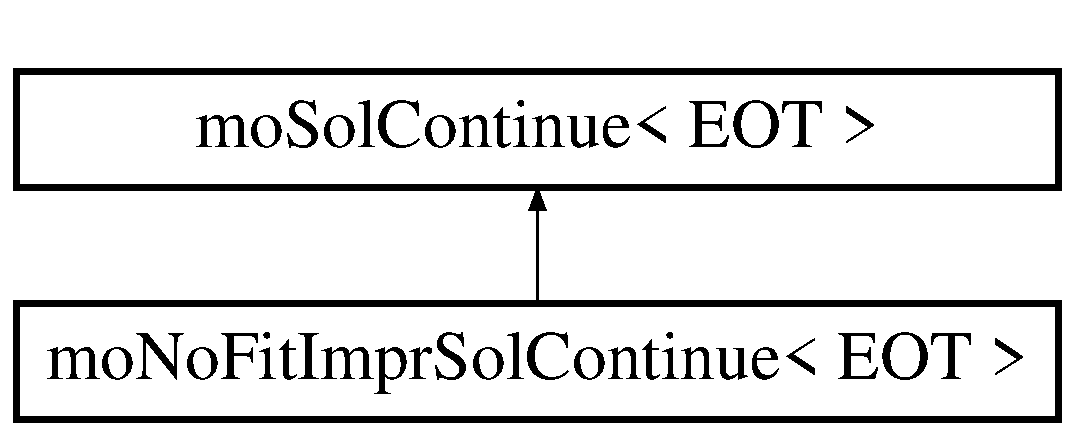
\includegraphics[height=4cm]{classmo_no_fit_impr_sol_continue}
\end{center}
\end{figure}
\subsection*{Public Types}
\begin{CompactItemize}
\item 
typedef EOT::Fitness {\bf Fitness}\label{classmo_no_fit_impr_sol_continue_64c184de66bb37d75d53aa600ac947b3}

\begin{CompactList}\small\item\em Alias for the fitness. \item\end{CompactList}\end{CompactItemize}
\subsection*{Public Member Functions}
\begin{CompactItemize}
\item 
{\bf moNoFitImprSolContinue} (unsigned int \_\-\_\-maxNumberOfIterationWithoutImprovment, bool \_\-\_\-maximization=true)
\begin{CompactList}\small\item\em Basic constructor. \item\end{CompactList}\item 
bool {\bf operator()} (const EOT \&\_\-\_\-sol)
\begin{CompactList}\small\item\em Function that activates the stopping criterion. \item\end{CompactList}\item 
void {\bf init} ()\label{classmo_no_fit_impr_sol_continue_21641c0a38a4501baae6133cbc591de4}

\begin{CompactList}\small\item\em Procedure which allows to initialise all the stuff needed. \item\end{CompactList}\end{CompactItemize}
\subsection*{Private Attributes}
\begin{CompactItemize}
\item 
unsigned int {\bf maxNumberOfIterationsWithoutImprovment}\label{classmo_no_fit_impr_sol_continue_9dbd725a2dab787f9f7b159b759e4834}

\begin{CompactList}\small\item\em Maximum number of iterations without improvment allowed. \item\end{CompactList}\item 
bool {\bf firstFitnessSaved}\label{classmo_no_fit_impr_sol_continue_ca3591e47a075b59e0826f31234c71ef}

\begin{CompactList}\small\item\em Flag that this is the first time that the fitness is used. \item\end{CompactList}\item 
{\bf Fitness} {\bf fitness}\label{classmo_no_fit_impr_sol_continue_3d3d2b43a4dd73e38689cc0018d44ee7}

\begin{CompactList}\small\item\em Current Fitness. \item\end{CompactList}\item 
bool {\bf maximization}
\begin{CompactList}\small\item\em Flag that indicate if there is a maximization (true) or a minimization (false) of the fitness value. \item\end{CompactList}\item 
unsigned int {\bf counter}\label{classmo_no_fit_impr_sol_continue_46fc008a8f7cd06dcaaeb4016b433adb}

\begin{CompactList}\small\item\em The iteration couter. \item\end{CompactList}\end{CompactItemize}


\subsection{Detailed Description}
\subsubsection*{template$<$class EOT$>$ class moNoFitImprSolContinue$<$ EOT $>$}

One possible stop criterion for a solution-based heuristic. 

The stop criterion corresponds to a maximum number of iterations without improvement. 



Definition at line 21 of file moNoFitImprSolContinue.h.

\subsection{Constructor \& Destructor Documentation}
\index{moNoFitImprSolContinue@{moNoFitImprSolContinue}!moNoFitImprSolContinue@{moNoFitImprSolContinue}}
\index{moNoFitImprSolContinue@{moNoFitImprSolContinue}!moNoFitImprSolContinue@{moNoFitImprSolContinue}}
\subsubsection{\setlength{\rightskip}{0pt plus 5cm}template$<$class EOT$>$ {\bf moNoFitImprSolContinue}$<$ EOT $>$::{\bf moNoFitImprSolContinue} (unsigned int {\em \_\-\_\-maxNumberOfIterationWithoutImprovment}, bool {\em \_\-\_\-maximization} = {\tt true})\hspace{0.3cm}{\tt  [inline]}}\label{classmo_no_fit_impr_sol_continue_979c991cbae53e1fd596964837c8d32d}


Basic constructor. 

\begin{Desc}
\item[Parameters:]
\begin{description}
\item[{\em \_\-\_\-maxNumberOfIterationWithoutImprovment}]The number of iterations without fitness improvment to reach for stop. \item[{\em \_\-\_\-maximization}]Indicate if the the aim is to maximize or minimize the fitness. \end{description}
\end{Desc}


Definition at line 34 of file moNoFitImprSolContinue.h.

\subsection{Member Function Documentation}
\index{moNoFitImprSolContinue@{moNoFitImprSolContinue}!operator()@{operator()}}
\index{operator()@{operator()}!moNoFitImprSolContinue@{moNoFitImprSolContinue}}
\subsubsection{\setlength{\rightskip}{0pt plus 5cm}template$<$class EOT$>$ bool {\bf moNoFitImprSolContinue}$<$ EOT $>$::operator() (const EOT \& {\em \_\-\_\-sol})\hspace{0.3cm}{\tt  [inline, virtual]}}\label{classmo_no_fit_impr_sol_continue_dbd663623cae56ec76ee504ecb226fed}


Function that activates the stopping criterion. 

Indicates if the fitness has not been improved since a given number of iterations (after a minimum of iterations). \begin{Desc}
\item[Parameters:]
\begin{description}
\item[{\em \_\-\_\-sol}]the current solution. \end{description}
\end{Desc}
\begin{Desc}
\item[Returns:]true or false. \end{Desc}


Implements {\bf eoUF$<$ const EOT \&, bool $>$}.

Definition at line 45 of file moNoFitImprSolContinue.h.

References moNoFitImprSolContinue$<$ EOT $>$::counter, moNoFitImprSolContinue$<$ EOT $>$::firstFitnessSaved, moNoFitImprSolContinue$<$ EOT $>$::fitness, moNoFitImprSolContinue$<$ EOT $>$::maximization, and moNoFitImprSolContinue$<$ EOT $>$::maxNumberOfIterationsWithoutImprovment.

\subsection{Member Data Documentation}
\index{moNoFitImprSolContinue@{moNoFitImprSolContinue}!maximization@{maximization}}
\index{maximization@{maximization}!moNoFitImprSolContinue@{moNoFitImprSolContinue}}
\subsubsection{\setlength{\rightskip}{0pt plus 5cm}template$<$class EOT$>$ bool {\bf moNoFitImprSolContinue}$<$ EOT $>$::{\bf maximization}\hspace{0.3cm}{\tt  [private]}}\label{classmo_no_fit_impr_sol_continue_73295d6a4ad437b0ab06848ac24698c4}


Flag that indicate if there is a maximization (true) or a minimization (false) of the fitness value. 

It can be interesting to know this information because some solution-based metaheuristics can generate solutions wiht a fitness that is worse that the best known fitness (in this case, the counter is not reinitialized). 

Definition at line 96 of file moNoFitImprSolContinue.h.

Referenced by moNoFitImprSolContinue$<$ EOT $>$::operator()().

The documentation for this class was generated from the following file:\begin{CompactItemize}
\item 
moNoFitImprSolContinue.h\end{CompactItemize}
